\subsection{スマホアプリによるビーコンと実デバイスによるビーコンの併用}


実デバイスによるビーコンはメンバの利便性が低く可用性に問題がある.
可用性とは,メンバの在室情報が長期にわたり継続的に記録される能力と定義する.
実デバイスによるビーコンを利用する場合,高い可用性を維持するにはバッテリ交換に配慮する必要がある.
そこで既存研究ではバッテリ切れが発生した場合,管理者がメンバにSlackを用いて
通知しバッテリ交換を催促していた.
しかし交換されない状況が存在した.
これは通知による催促が不確実かつ即時性がないためである.
通知は一定期間の在室がない場合にバッテリ切れの可能性があると見做して通知している.
そのため通知の正確性が低い上,バッテリ切れに対してタイムラグがある.
また交換作業がメンバに委ねられており,その手間による利便性が低くバッテリ切れの放置が発生した.


上記の問題のアプローチとしてメンバの利便性を向上させるため,スマホアプリによるビーコン動作(以下,スマホビーコン)を行った.
BLEビーコンの代替としてスマートフォンを利用可能にするとバッテリ交換の手間が削減される.
またスマートフォンユーザにとってスマートフォンはコミュニケーションツールとしての用途からバッテリ切れを配慮する傾向が強い.
よって実デバイスによるビーコンと比べてスマホビーコンはバッテリが維持されやすく利便性が向上すると考えた.

スマホビーコンは基本的にバックグラウンドに常駐させる利用法を想定し実装した.
既存研究では,メンバに実デバイスによるビーコンを携帯させ,能動的な記録動作の必要がない.
バックグラウンドに常駐させる方式は実デバイスによるビーコンと同様に能動的な記録動作を必要としないため同等の利便性がある.
スマートフォンの画面表示が可能な利点を利用し,スマートフォンの通知領域に動作状況を表示した.
通知領域への表示はスマホビーコンの動作と連携しており,動作中に表示される.
メンバにとって実デバイスによるビーコンは動作の把握が困難であったが,通知領域への表示により動作の把握が可能になった.
そのためビーコン動作の停止に気が付きやすく,メンバによる再起動が行われた場合,可用性の向上が期待できる.





スマホビーコンのみを利用する場合,様々な状況下でメンバの継続した利用が困難であるため,実デバイスによるビーコンと併用できるシステムとした.
普段から継続的に利用するメンバにとっては,実デバイスによるビーコンは先述の通りバッテリ交換の手間がある.
スマホビーコンはそのようなメンバにとっては,バッテリ交換の手間がないため有用である.
しかしスマホビーコンのインストールに抵抗があるメンバやインストールができないメンバも想定される.
例としてはスマートフォンを所有していないメンバ,スマホビーコンの利用に伴うバッテリ消費が気になるメンバなどが挙げられる.
これらの問題は実デバイスによるビーコンとスマホビーコンのハイブリッド化によって解決できる.
スマホビーコンで利用するUUIDを実デバイスによるビーコンで利用するUUIDと同じ値に設定し同じメンバの在室情報を記録している.
この方法は表1に示す通りスマホビーコンか実デバイスによるビーコンの少なくとも片方を携帯していれば記録できるため継続的にデータを記録する観点から見ても有用である.
% \begin{table}[tbh]
%   \centering
%   \caption{各ビーコンのみ対応時とハイブリッド対応時の比較}
%   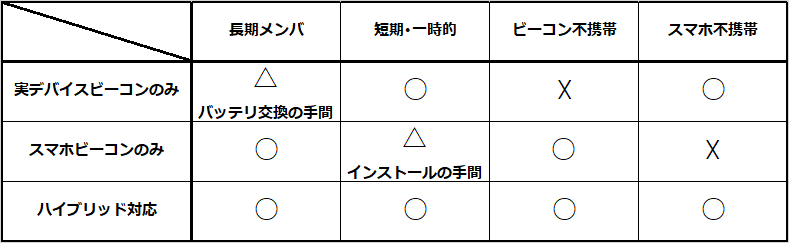
\includegraphics[width=9cm]{image/table.png}
%   \label{multipleBPM}
% \end{table}
\begin{table}[tbh]
    \caption{各ビーコンのみ対応時とハイブリッド対応時の比較}
    \scalebox{0.55}{
        \begin{tabular}{|c|c|c|c|c|}
                \hline
                 & 長期メンバ & 短期・一時的 & スマホ不携帯 & ビーコン不携帯 \\ \hline
                実デバイスビーコンのみ & \begin{tabular}[c]{@{}c@{}}△\\ バッテリ交換の手間\end{tabular} & ○ & ☓ & ○ \\ \hline
                スマホビーコンのみ & ○ & \begin{tabular}[c]{@{}c@{}}△\\ インストールの手間\end{tabular} & ○ & ☓ \\ \hline
                ハイブリッド対応 & ○ & ○ & ○ & ○ \\ \hline
                \end{tabular}
    }
    \label{multipleBPM}
\end{table}

% \begin{table}[tbh]
%     \scalebox{0.25}[0.25]{
%     \begin{tabular}{|c|c|c|c|c|}
%     \hline
%      & 長期メンバ & 短期・一時的 & スマホ不携帯 & ビーコン不携帯 \\ \hline
%     実デバイスのみ & \begin{tabular}[c]{@{}c@{}}△\\ バッテリ交換\end{tabular} & ○ & ☓ & ○ \\ \hline
%     スマホのみ & ○ & \begin{tabular}[c]{@{}c@{}}△\\ インストール\end{tabular} & ○ & ☓ \\ \hline
%     ハイブリッド対応 & ○ & ○ & ○ & ○ \\ \hline
%     \end{tabular}
%     }
%     \end{table}
